\documentclass[12pt,a4paper,oneside,titlepage]{article}
\usepackage[utf8]{inputenc}
\usepackage[english]{babel}
\usepackage{amsmath}
\usepackage{amsfonts}
\usepackage{amssymb}
\usepackage{textcase} 
\usepackage{tocloft}
\usepackage{lastpage}
\usepackage{graphicx}

\usepackage[font=small,labelfont=bf,labelsep=space]{caption}
\captionsetup{%
  figurename=Fig.,
  tablename=tab.
}

\graphicspath{{images/}}
\usepackage{tikz}
\usetikzlibrary{arrows,positioning}
\usetikzlibrary{shapes, arrows}
\usepackage[left=3.5cm,right=1cm,top=2cm,bottom=2cm]{geometry}
\author{Kostenko}
\setcounter{tocdepth}{3}%для глубины страницы содаржения
\renewcommand{\baselinestretch}{1.25}
\renewcommand{\cftsecleader}{\cftdotfill{\cftdotsep}} % точки в содержании для секций
\bibliographystyle{unsrt}
\begin{document}
{
\thispagestyle{empty}
\newpage
\centering

\textbf{
National Research University Higher School of Economics\\
}
Faculty of Business Informatics

School of Software Engineering

Software Management Department

\vfill


\begin{large}
\MakeTextUppercase{
An Application for Dynamic Object Identification Based on Lucas-Kanade Algorithm
}
\end{large}


\vfill

\begin{tabular}{lr}
Student: & Kostenko Dmitry \\
Group: & 472SE \\
Argument Consultant: & Prof. Ivan. M. Gostev, PhD \\
Style and Language Consultant: & Tatiana A. Stepantsova
\end{tabular}

\vspace{\fill}

Moscow\\ \number\year
\clearpage
}

\section*{Abstract}
{
%В данной статье описывается подход к обнаружению и подсчету транспортных средств на атодорогах.
%Он основан на дифференциальном методе вычисления оптического потока, предложенном Лукасом и Канаде.
%Отличие данного метода от других состоит в том, что нет необходимости подготавливать модель фона.
%Так же описываются достоинства и недостатки данного подхода.

In this paper a method for detecting and counting vehicles on a highway is described. 
It is based on a differential method of counting the optical flow suggested by Lucas and Canade \cite{lucaskanade}. 
This method is different from other methods in a way that it does not require a pre-made model of the background. 
Advantages and disadvantages of such an approach are also described.


}





{
\newpage
\centering
\tableofcontents
}











\newpage
\section{Introduction}
%Nowadays it is possible to notice high grow of vehicles in all Russian cities.
%According to DPS data annual growth of cars number is 110 - 120 thousand.
%As a result the significance of traffic conjunction problem increases.
%It causes higher fuel usage 
%One of the decisions of the problem is installation of Intelligent Transportation System (ITS).
%ITS ranges from simple traffic light control systems to systems which register velocity of vehicles flow, control traffic flow and recognition of the violations.
%Such systems can perform the following tasks:
%\begin{enumerate}
%  \item ensuring maximum traffic capacity;
%  \item reducing road accidents and monitoring human factor;
%  \item collecting information about traffic jams from the vehicle flow and informing its participants;
%  \item environment protection as a result of real-time monitoring of road situation and well timed decisions making.
%\end{enumerate}

Nowadays a significant growth of the vehicles amount can be observed in all Russian cities.
According do the Russian highway patrol data, this growth is approximately a hundred thousand new cars per year.
Taking into account the fact that almost no new highways appear, we can easily come to a conclusion that the traffic conjunctions problem is a direct result of this annual growth.
Another problem that arises as a side effect of the jammed highways is an increase in fuel usage.
A good solution of these problems can be installing an Intelligent Transportation System (ITS).
These systems range from rather simple implementations which are able to control traffic lights to sophisticated solutions that are capable of registering the vehicle flow velocity and predicting violations.
These are the tasks, which are usually assigned to these systems:
\begin{enumerate}
	\item ensuring maximum traffic capacity;
	\item reducing the amount of accidents on the highway and monitoring the human factor;
	\item collecting the information about the traffic jams from the vehicle flow and informing its participants;
	\item environment protection as an indirect result of real-time monitoring of situation on the roads.
\end{enumerate}


ITS can contain various sensors from the ones that are capable of detecting heat to the ultrasonic ones.
Manual processing of a significant amount of data which is received from these sensors is not applicable in the real-life situations.
As a consequence, a vital necessity of automation of the process and decision making, based the information gathered during this process, arises.
Automatic vehicle detection in this video monitoring is a complex objective of computer vision.
On of the tasks of such a system is to count vehicles on the highway.
In its turn, it is divided into subtasks of computer vision, such as foreground retrieving (vehicles) and tracking in the next frames.
This paper offers an overview of an approach which is related to automatic tracking of moving vehicles.
The only source of data used by this approach is a camera video recording.
The first chapter of the present graduation paper offers an overview of existing solution in the field of video monitoring.
Problem statement and requirements to the algorithm under development are covered in the second chapter.
The third chapter deals with description of methods and algorithms.
And finally, the brief exploration of expected results will be introduced.


%В наше время наблюдается высокие рост количества транспортных средств во всех городах России.
%По данным ГИБДД только в Москве ежегодный прирост автомобилей составляет 110 - 120 тысяч.
%В результате проблема заторов автотранспортных дорог становится более острой.
%Как следствие увеличивается расход топлива, уровень загрязнения окружающей среды и время пути каждого автомобилиста.
%Одним из решений данной проблемы является установка городской интелектуальной транспортной системы (ИТС).
%ИТС варьируются от простых систем регулирования светофоров, до систем регистрации скорости потоков транспортных средств, контроля автомобильного потока и распознования фактов нарушений.
%(http://ru.wikipedia.org/wiki/Интеллектуальная_транспортная_система)
%Такие системы позволяют решать следующие задачи.
%1) Обеспечение максимальной пропускной способности.
%1) Безопасность. Основная цель — снижение аварийности на дорогах. Сюда же входит мониторинг природных катаклихмов и человеческого фактора.
%2) Мобильность. Сбор информации о пробках от движущихся в потоке автомобилей и информирование участников движения.
%3) Защита окружающей среды. Снижение ущерба окружающей среде от автотранспорта посредством мониторинга ситуации в реальном времени и своевременного принятия решений.
%ИТС может содержать в себе датчики различных типов, от тепловых до ультразвуковых.
%Ручная обработка гигантского объема данных, поступающих от всех сенсоров таких систем непрактична.
%Поэтому появляется необходимость автоматизировать обработку данных и заключения выводов на основе них.
%Автоматическое обнаружение транспортных средств в данных видеонаблюдения является комплексной задача в компьютерном зрении.
%Одной из задач такой системы является подсчет транспортных средств на автодороге.
%Которая в свою очередь тоже разбивается на подзадачи компьютерного зрания, такие как: выделение объектов переднего плана (автомобилей) и отслеживание их положения в последующих кадрах.
%В данной статье мы описываем подход к решению задачи автоматического отслеживания движущихся транспортных средств и их подсчета.
%Где единственным источником данных о ситуации на автодороге является видеокамера. 
%Краткое содержание последующих глав:
%3) Обзор существующих решений в области видеонаблюдения на автодорогах.
%4) Постановка задачи и формулирование требований к разрабатываемому алгоритму.
%5) Изложение методов и алгоритмов решения поставленной задачи
%6) Краткое содержание планируемых рещультатов работы и выводы.

















\newpage
\section{Related work}
%В данной главе представлен краткий обзор существующих решений в области видеонаблюдения на автодорогах.
%В мире существует только одна всеобъемлющая архитектура ИТС. Предложенная транспортным департаментом США инициатива, направленная на создание единого информационного пространства, объединяющего автомобили, дорожное оборудование, диспетчерские залы и центры обработки данных по всей стране. Данная транспортная система запатентована правительством США.
%(http://www.iteris.com/itsarch/documents/physical/physical.pdf)
%В городе Москве в 2012 году начала свое действие российская ИТС.
% http://mskit.ru/news20/no117891/
%Существуют аналоги, частично реализующие функционал ИТС США.
%Данные системы являются закрытыми.
%Но существует множество проектов с меньшим масштабом и функционалом имеющие открытые описания применяемых методов.
%Как было отмеченно, одной из задач таких систем является подсчет количества транспортных средств на автодороге.
%И чаще всего алгоритм подсчета транспортных средств на автодороге выглядит так:
%1) создать модель фона
%2) вычесть из текущего изображения модель фона и получить движущиеся объекты переднего плана (транспортные средства)
%3) посчитать количество транспортных средств, пересекающих линию интереса
%4) обновить модель фона
%Наша работа отличается тем, что мы предлагаем альтернативный вариант подсчета количества транспортных средств без заранее смоделированного фона.
%Используя наш подход выявление транспортных средст базируется на сумме разностей рядом стоящих кадров видеопоследовательности и выделения связных компонент на изображении.

In this section a short review of existing highway video surveillance solutions is presented.
There is only one full ITS architecture, developed by the transportation department of the US. It focuses on creating a unified information environment, that connects automobiles, road equipment, dispatch centres,  and data centres around the country. This system has been patented by the US government.

There are several analogues around the world that are based on the US system. In 2012 a Russian ITS was rolled out in Moscow. All of these systems are commercial and there are no ways of analysing there methods.
However, there are also several open-source projects of smaller scale.
As has been mentioned before, one of the main tasks of such systems is counting vehicles on the highway.

Most of the times the vehicle counting algorithm consists of the following steps:


\begin{enumerate}
  \item create the background model;
  \item subtract this model from the current image and obtain all moving objects of the foreground (vehicles);
  \item count the amount of vehicles that has crossed the line of interest;
  \item update the model of the background.
\end{enumerate}



Examples of such an approach: ****\

Our work uses a different approach. We suggest an alternative method for counting vehicles without the pre-modelled background.
It is based on the differences sum  of the neighbouring frames of a video sequence and highlighting the connected areas.



























\newpage
\section{Problem statement}
%Резальтатом данной главы будет являтся список требований к алгоритму.
%Для формальности приведем некоторые определения.
%Т.к. видео - это последовательность кадров, то в каждый момент времени мы имеем один кадр, называемый текущим.
%Если кадр i - текущий кадр, то кадр (i-1) - предыдущий.
%Объектами переденго плана будем считать любые движущиеся объекты (транспортные средства, деревья, люди).
%Определение объекта, как движущегося, зависит от характеристик камеры и окружающей обстановки.
%Поэтому движущимися объектами назовем те объекты, которые меняют свое положение на текущем кадре, относительно предыдущего кадра.
%Движущийся объект перед камерой или движущиеся камера в неподвижной обстановке ведет к изменения изображения.
%Изображение видимого движения объекта называется оптическим потоком.
%Существует несколько методов вычисления оптического потока.
%Лукас и Канаде предложили дифференциальный подход.
%О нем будет рассказано позже.
%Теперь перейдем к постановке задачи.
%Одна из наиболее важных задач в видео наблюдении состоит из идентификации объекта интереса и отслеживание его траектории в последующих кадрах.
%Эта задача может быть разбита на подзадачи.
%Первое, необходимо обнаружить объекты интереса или объекты переднего плана.
%Обнаружение объектов интереса подразумевает под собой отделение переднего плана от фона на изображении.
%После того, как мы это сделали мы получим бинарную карту движущихся объектов на изображении.
%Далее необходимо понять, какие из движущихся объектов являются автотранспортными средствами, а какие не являются таковыми. 
%Так как на изображении могут двигаться не только объекты переднего плана, но и объекты заднего плана (например ветви деревьев), то появляется необходимость борьбы с данным явлением.
%Для этого ограничим на изображении область, в которой мы и будем вести видеонаблюдение. %рисунок
%Такой областью лучше всего выделить хорошо просматриваемый промежуток автодороги.
%Затем следить за изменениями координат обектов интереса в последующих кадрах.
%Для вычисления оптического потока необходимо сделать несколько предположений.
%1) изображение - это непрерывная функция от двух переменных;
%2) яркость объекта остается неизменной в небольшой промежуток времени;
%3) отслеживаеммый объект на новом кадре будет расположен на небольшом расстоянии относительно предыдущего кадра.
%Первое предположение дает нам возможность использовать методы математического анализа и позволяет производить матемстические операции над изображением.
%Второе предположение существует потому, что мы живем в реальном мире, в котором  обхекты не могут мгновенно перемещаться на большие расстояния.
%Третье предположение необходимо потому что мы не сможем без него отслеживать объект.


In this chapter we will state the set of requirements for the algorithm.
As a formality we will state several definitions first.
As any video is a sequence of frames, every moment in time we have one frame called the current frame.
If the current frame is defined as i, the previous frame will be defined as (i-1).
We will consider all the moving objects such as vehicles, trees, humans as the foreground.
Whether the object is considered as a moving one depends on the camera properties and the environment.
So we define moving objects as the ones that shift their position in the current frame, relatively to previous frame.
When the camera moves, or the object in its focus, it leads to the image changes.
The description of the movements which can be seen is called the optical flow.
There are several methods for calculating this flow.
Lucas and Kanade developed one of them, using differential approach \cite{lucaskanade}.
It will be described later in this paper.
Now let us move to the problem statement.
One of the most important problems of video surveillance is identifying the object of interest and following its trajectory through the sequence of the following frames.
This problem can be partitioned into several sub-problems.
In the beginning it is necessary to find the objects of interest, which can also be called the foreground objects.
Finding these objects involves separation of the foreground from the background of the image.
As a result we get a binary map of the moving objects.
After that we need to separate vehicles from other moving objects such as trees or humans. 
For doing so we limit the area in which we will track movement.
%и назовем ее областью интереса
A good choice will be a well-observed part of a highway. 
Then we need to track the changes in objects of interest coordinates in the following frames.

To calculate the optical flow we need to make several assumptions:
\begin{enumerate}
  \item An image is a continuous function of two variables. This will let us use mathematical analysis, and also carry out mathematical operations with the image;
  \item The brightness of an object remains constant in a short period of time. Without this assumption we will not be able to track the object;
  \item The location of the object of interest will not change a lot relatively to the previous frame. This is due to the fact that in real life objects do not move with the speed of light.
\end{enumerate}

 



Let us state the problem: counting the amount of vehicles which appear in a certain area of interest.

We can also formulate the following algorithm requirements:
1) working without any specific data about the highway, or the images that are going to be processed;
2) real-time processing of the data flow;
3) not requiring a significant amount of computational power. The minimal hardware requirements will be proposed in the specification. At the time of writing this paper these requirements are impossible to describe.

Now let us move to the descripton of the algorithm.

%Сформулируем задачу: посчитать количество автомобилей, пересекающих область интереса.

%Теперь мы можем сформулировать требования к алгоритму:
%1) Работать без каких-либо предварительных данных об автодороге,
%2) Обработка потока данных в реальном времени
%3) Не должен требовать высоких вычислительных мощностей. Минимальные требования к оборудованию будут предложены в техническом задании, на стадии написания данной бумаги их невозможно сформулировать.


%Перейдем к изложению алгоритма.





























\newpage
\section{Algorithm}
%В данной главе раскрывается подход к обнаружению и подсчету транспортных средств на атодорогах.
%Т.к. видео - это последовательность кадров, то в каждый момент времени мы имеем одно изображение.
%При получении нового кадра, сперва необходимо избавиться от шумов.
%Для этого сгладим изображение фильтром Гаусса. %ссылка на гауса
%Так как в дальнейшем мы не будем использовать информацию о цвете объектов, то для уменьшения количества избыточной информации переведем изображение из цветовой модели RGB в градации серого. %сказать каким алгоритмом
%Так же, для увеличения скорости обработки изображения нужно уменьшить его размер.
%Но это возможно сделать только в том случвае, если характеристики камеры позволяют это сделать. 
%Например, если камера снимает с разрешением большим чем 640x480, то можно его уменьшить до 640×480, что увеличит скорость обработки каждого кадра.
%После всех операций предобработки кадров выделим объекты переднего плана.



In the following chapter an approach to the task of vehicles on motor ways detection and counting will be revealed.

As a video is a frame sequence, at every moment only one frame is available.
In the beginning, it is necessary to eliminate a noise of each frame.
Gauss filter must be applied in order to perform this.
The information about object color seems to be not in use in further.
Therefore it will be appropriate to transform the image from RGB color space to grayscale.
Also, for the sake of increasing the processing performance it is necessary to reduce the size of the image.
But it is possible only if the camera allows to do so.
For instance, if the camera shoots with a resolution of more than 640 by 480 pixels, every frame of the video stream can be reduced to this resolution to increase the processing performance of every frame.
After all of the images pre-processing procedures, the foreground objects are detected.






















\subsection{Allocation of foreground objects}
%Целью метода, описанного в данном блоке, является получение положений объектов, относящихся к переднему плану.
%Традиционные алгоритмы получения объектов переднего плана основаны на методе попиксельного вычитания изображений.
%Но у данного метода есть недостаток.
%С помощью него мы можем получить большое количество несвязных областей. %показать картинку
%Поэтому, для получения более связных областей, необходимо модифицировать данный метод.
%Сперва разобьем каждый кадр на непересекающиеся блоки.
%Оптимальный размер блока определяется империческии и зависит от характеристи камеры и окружающей обстановки.
%Поэтому, для начала, зададим размер блока равный 3х3 пикселей.
%Затем попиксельно вычтем предыдущий кадр из текущего.
%В конце, отфильтруем пиксели каждого блока у полученной разности изображений таким образом:
%если количество пикселей в каждом блоке, относящихся к объектам переднего плана, превышает заданный порог, то будем считать, что блок принадлежит переднему плану.
%В инном случаем будем считать обратное.
%В результате мы получим бинарное изображение объектов переднего плана.%показать картинку
%Но на данном изображении могут присутствовать шумы.
%Поэтому необходимо обработать изображение морфологическими операциями.
%Применим эррозию, а затем наращивание. % dilation
%Так же необходимо заметить, что метод вычитания предыдущего кадра из текущего дает хороший отклик на границе движущегося объекта.
%Но в оласти движущегося объекта наблюдается обратный эффект. %показать картинку
%В случае, когда транспортное средство имеет большие размеры, вероятность определить транспортное средство, как объект переднего плана, существенно уменьшается.
%Чтобы избежать подобного эффекта введем еще 2 понятия: краткосрочная модель переднего плана и долгострочная модель  переднего плана.
%Краткосрочной моделью переднего плана является такая модель, которая получается в результате применения последовательности действий, описанных выше.
%Долгосрочной моделью переднего плана назовем попиксельную сумму N моедлей переднего плана, где N - натуральное число и больше 1.
%N зависит от характеристик камеры и окружающей среды вычисляется империческим путем.
%Т.к. отслеживаемые объекты движутся, то при вычислении долгосрочной модели переднего плана мы получим более свзные области предполагаемых транспортных средств. % показать кратинку
%На изображении видно, что область объекта может разделиться на несколько областей.
%Для уменьшения количества связных областей применим морфологическую операцию наращивание.



The primary goal of the method, described in this section, is retrieving the foreground objects location.
The traditional algorithms of retrieving the foreground objects location are based on pixel-by-pixel frame difference method.
But this method also has several disadvantages.
This method's application might lead to the enormous amount of isolated areas (Fig. \ref{ris:pixel_by_pixel}).

\begin{figure}[h]
  \center{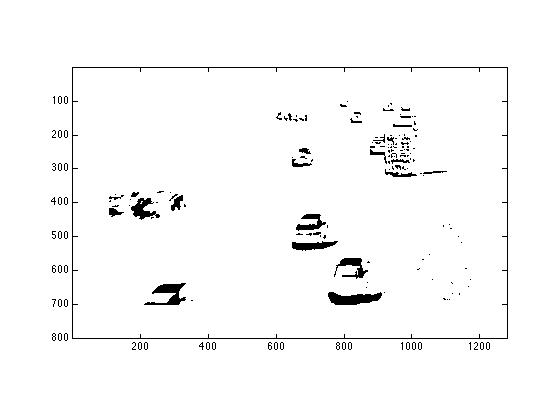
\includegraphics[width=10cm]{1.jpg}}
  \vspace{-5ex}
  \caption{\textit{Pixel-by-pixel frame difference method.}}
  \label{fig:pixel_by_pixel}
\end{figure}

For this reason, this method must be modified to avoid this disadvantage and to make these areas connected with each other.
At first, each frame has to be divided into blocks which do not overlap.
The optimal size of a block is found empirically and depends on characteristics of the camera and the environment.
That is why in the beginning the standard size will be assigned to each block - 3x3 pixels.
In Fig. \ref{fig:fig2}.

\begin{figure}[h]
  \center{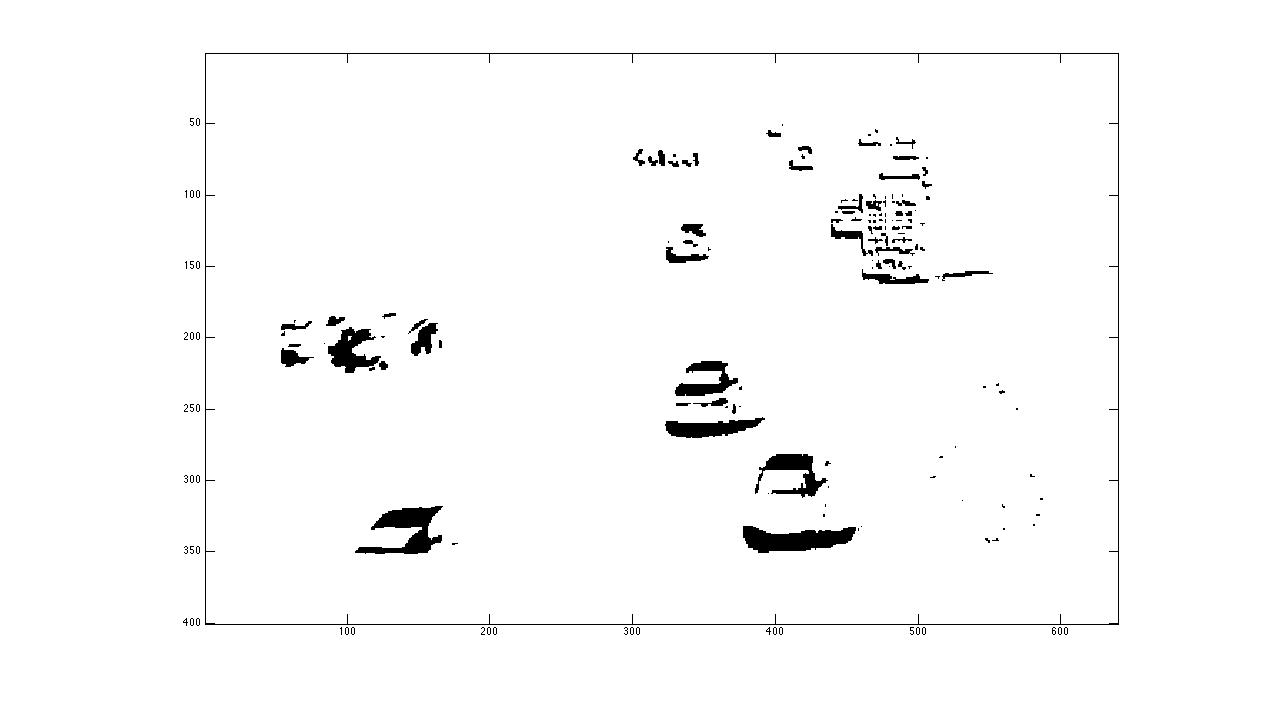
\includegraphics[width=10cm]{2.jpg}}
  \vspace{-5ex}
  \caption{\textit{The result.}}
  \label{fig:fig2}
\end{figure}


After that the previous frame is subtracted from the current frame.
Then every pixel block of the result is filtered in the following way:
if the amount of foreground objects pixels in every block is more than some pre-defined threshold, this block is considered to be the foreground
otherwise, it is considered to be the background

As a result we get the binary image of the foreground objects.
But this image is not going to be perfect, it will definitely have noise.
For that reason the image must be processed using morphological operations.
These operations are the following: erosion and dilation.

It is necessary to consider that the method of subtracting the previous frame from the current frame gives good response near the moving object border. 
However, inside the objects borders the response is NOT SO GOOD.
If the vehicle is relatively large, the probability of its recognition as an object of the foreground is low.

To get rid of this effect let us consider two definitions: sort-term model of the foreground and long-term model of the foreground.

The short-term model is the model which we get, after applying the steps stated above.
The long-term model is the pixel-by-pixel sum of N previous short-term foreground models, where N is a positive integer and more than 1 (Fig.\ref{fig:frames_and_sum}).
N is found empirically and depends on characteristics of the camera and the environment.




\begin{figure}[h]
	\begin{minipage}[h]{0.19\linewidth}
		\center{
\includegraphics[width=1\linewidth]{frame1} \\ a)}
	\end{minipage}
	\hfill
	\begin{minipage}[h]{0.19\linewidth}
		\center{
\includegraphics[width=1\linewidth]{frame2} \\ b)}
	\end{minipage}
	\hfill
	\begin{minipage}[h]{0.19\linewidth}
		\center{
\includegraphics[width=1\linewidth]{frame3} \\ c)}
	\end{minipage}
	\hfill
	\begin{minipage}[h]{0.19\linewidth}
		\center{
\includegraphics[width=1\linewidth]{frame4} \\ d)}
	\end{minipage}
	\hfill
	\begin{minipage}[h]{0.19\linewidth}
		\center{
\includegraphics[width=1\linewidth]{frame_sum} \\ e)}
	\end{minipage}

	\caption{\textit{(a) - first frame; (b) - secind frame; (c) - third frame; (d) - fourth frame; (e) - sum of all frames.}}
	\label{fig:frames_and_sum}
\end{figure}



As the objects that we want to track are moving, calculating the long-term model of  the foreground we get the object regions, which is more connected.
As can be seen from Fig.\ref{fig:fig3} the object region can be separated into several regions.
To reduce the amount of these regions we use the dilation operation with pre-defined window.


\begin{figure}[h]
  \center{
\includegraphics[width=0.2\linewidth]{frame4}}
  \caption{\textit{Object, separated into several regions.}}
  \label{fig:fig3}
\end{figure}














\subsection{Selection of connected regions}
%В данной главе излагается метод сегментации объектов переднего плана.
%После того, как мы получили бинарную карту объектов переднего плана, то необходимо пронумеровать их.
%Будем использовать простейший алгоритм сегментации.
%Итак, пусть у нас имеется бинарное изображение.
%В нашем случае 0 - это фон, а 1 - потенциальное транспортнгое средство.
%В данном случае разметка является однозначной при фиксированном виде связности. 
%Связным множеством будем называть такое множество пикселей, у каждого пикселя которого есть хотя бы один сосед, принадлежащий данному множеству.
%Существует 2 вида связности:
%1) 4 связность - соседями для пикселя считаются 4 пикселя: сверху, слева, справа, снизу.
%2) 8 связность - соседями для пикселя считаются 8 пикселей, т.е. все к нему прилежащие, в том числе и по диагонали.
%Мы будем использовать 8-ми связность.

After creating the binary map of the foreground objects, it is necessary to give every object a certain number.
A straightforward segmentation algorithm is used.
Suppose, we obtained the binary image.
In our case white pixels stand for the background, and black pixels stand for the potential vehicles.
The mapping from the original image to the segmented image is mono-semantic. 
We will call an array of pixels connected if and only if each pixel has at least one neighbouring pixel belonging to this array.
There are two ways for pixels to be connected:

\begin{enumerate}
  \item 4 connected (Fig. \ref{ris:connections} (a)) - the neighbours of the pixel are only the following pixels: the one above, the one below, the one to the right and the one to the left of it;
  \item 8 connected (Fig. \ref{ris:connections} (b)) - the neighbours of the pixel are the pixels above, below, to the right, to the left, and the diagonal pixels.
\end{enumerate}



\begin{figure}[h]
\begin{minipage}[h]{0.49\linewidth}
\center{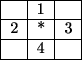
\includegraphics[width=0.2\linewidth]{four-svyaznost.png} \\ a)}
\end{minipage}
\hfill
\begin{minipage}[h]{0.49\linewidth}
\center{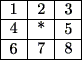
\includegraphics[width=0.2\linewidth]{eight-svyaznost.png} \\ b)}
\end{minipage}
\caption{\textit{(a) 4-connected, (b) 8-connected}}
\label{ris:connections}
\end{figure}



In our approach the 8 connected way is used, because it gives a significant raise in precision.
There are generally known two methods of image marking: recursive and iterative.
The shortcomings of the recursive approach are the following:
\begin{enumerate}
  \item a great amount of memory is needed for it;
  \item it is rather slow, compared to the iterative method.
\end{enumerate}
The iterative method is an alternative to the recursive approach. It can be often met in literature by the name of: "Sequential scanning algorithm".
Let us present it in detailed steps:
\begin{enumerate}
  \item To be specific, we start processing the pixels of the image from the left-top corner, going from the top to the bottom and from the left to the right.
  \item While cycling through the pixels of the image we ignore the background pixels, and mark the current pixel with the color of the top-left neighbouring pixel.
\end{enumerate}

The idea behind this algorithm is to use a special mask, shaped like a corner, called the ABC mask. 
This mask can be seen in the Fig. \ref{fig:abc_mask}.
Going through the image with this mask is carried out in a top to bottom and left to right fashion.
It is assumed that there are no objects behind the image border, so it is possible for a B or a C to end up behind this border.
This requires an extra verification after the scanning.
Figure \ref{fig:abc_all_cases} shows five possible positions for the ABC mask on the image.

%Идея данного алгоритма основана на использовании уголка — ABC-маски, которая показана on Fig. \ref{fig:abc_mask}.
%Проход по изображению данной маской осуществляется слева-направо и сверху-вниз. 
%Считается, что за границей изображения объектов нет, поэтому, если туда попадают B или C — это требует дополнительной проверки при сканировании. 
%На рисунке 4 изображены 5 возможных позиций маски на изображении.



\begin{figure}[h]
  \center{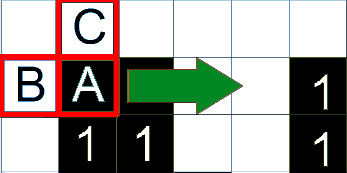
\includegraphics[width=0.3\linewidth]{abc_mask.jpg}}
  \caption{\textit{ABC-mask.}}
  \label{fig:abc_mask}
\end{figure}



\begin{figure}[h]
  \center{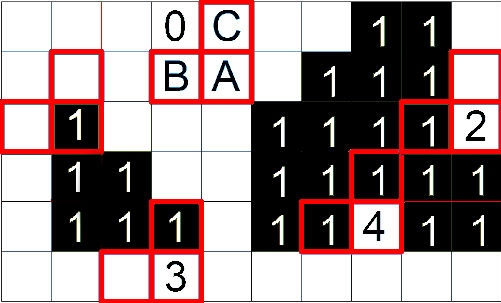
\includegraphics[width=0.3\linewidth]{abc_all_cases.jpg}}
  \caption{\textit{5 cases of ABC-mask.}}
  \label{fig:abc_all_cases}
\end{figure}


\begin{enumerate}
	\item Position 0, where all three components of the mask are not marked — in this case we simply skip the pixel.
	\item Position 1, where only the A element is marked — in this case we have found a new object which gets its own unique number.
	\item Position 2, where only the B element is marked — in this case we mark the current  A pixel with a number from B.
	\item Position 3, where only the C element is marked — in this case we mark the current  A pixel with a number from C.
	\item Position 4, here the B and C marks are connected and equivalent  and the A pixel can be marked with the number either from C or B. In some implementations the equivalence graph of such marks is created, with some explanations. We do not consider it necessary. We are going to do the following - in the case, where B is equal to C, we go back and mark all processed pixels marked as C with B. This process will be described in detail later in this paper. 
\end{enumerate}


%\begin{enumerate}
%	\item Позиция под номером 0, когда не размечены все три компонента маски — в этом случае мы просто пропускаем пиксель.
%	\item Позиция под номером 1, когда помечен только элемент A — в этом случае мы говорим о создании нового объекта — новый номер.
%	\item Позиция под номером 2, когда помечен элемент элемент B — в этом случае мы помечаем текущий пиксель A меткой, расположенной в B.
%	\item Позиция под номером 3, когда помечен элемент элемент С — в этом случае мы помечаем текущий пиксель A меткой, расположенной в С.
%	\item Позиция под номером 4, тогда мы говорим о том, что метки (номера объектов) B и C связаны — то есть эквивалентны и пиксель A может быть помечен либо как B либо как C. В некоторых реализация составляют граф эквивалентности таких меток, с последующим его разбором, однако на мой взгляд в это нет необходимости. Мы будем делать так — в том случае, если B не равно C то перенумеруем все уже обработанные пиксели помеченные как С в метку B. Но об этом в самом конце.
%\end{enumerate}
%Существует 2 известных метода разметки: рекурсивный и итеративный.
%Недостатком рекурсивного метода является медленная работа и большой расход памяти.
%Существует и итеративный метод, который в литературе часто встречается под названием "алгоритм последовательного сканирования". Опишем и его:
%Начинаем обход изображения, для определённости, из левого верхнего угла сверху вниз, справа налево. 
%При обходе пропускаем пиксели фона. 
%После того как мы обошли всю картинку, нам нужно совершить ещё один обход и произвести переразметку с учётом эквивалентности областей.
%В результате мы получим изображение, на котором каждая связная область помечена своим номером.
%Теперь необходимо отбросить области, которые не могут быть классифицированы, как транспортные средства.
%Для этого посчитаем количество пикселей у каждой области и отбросим те, у которых количество пикселей не превышает заранее установленный порог.
%Данный порог будет установлен империческим путем и будет зависить от характеристик камеры и от окружающей среды.
%На данном этапе написания работы мы не можем сказать, каким значением можно инициализировать данный порог.
%Поэтому просто проигнорируем его существование и будем считать, что все связные области в пределах области интереса являются транспортными средствами.




After processing the image, we need to go through the array of pixels again and do the marking procedure with the consideration of areas equality,
As a result, an image is obtained, where each connected area is marked with its own number.
Now we cut out the areas which can not be classified as vehicles.
To do so, we need to count the amount of pixels in each area. The areas in which the amount of pixels exceeds a certain threshold are eliminated.
This threshold is found empirically and will depend on the camera characteristics and the environment conditions.
At the time of writing we can not tell exactly what the threshold is going to be.
That is why, for now we will just ignore it and consider all of the connected areas to be the vehicles that we are looking for. 









\subsection{Vehicle tracking and counting}
%здесь описание отслеживания существующих такчек и +1 к счетчику
%После того, как мы получили связные области (которые являются транспортными средствами) на текущем кадре, нам необходимо понять, какие из этих объектов новые, а какие уже существовали на прошлом кадре.
%Будем считать, что положение связной области определяется, как координаты центра связной области.
%Такой центр вычисляется как среднее значение всех х-координат и y-координат пикселей, принадлежащих области.
%Т.е. задача формулируется таким образом: необходимо сопоставить текущие связные области с такими же на предыдущих кадрах или инициализировать новые.
%Ранее мы сделали несколько ключевых предположений.
%Одним из них было продположение о том, что атвомобиль на текущем кадре сдинулся на небольшое расстояние отоносительно себя на предыдущем кадре.
%Таким образом, храня положения цетров связных областей мы можем найти ближаший центр данной области на текущем кадре к этой же области на предыдущем кадре, используя подход, предложенный Лукасом и Канаде.
%Основное идеей данного метода является нахождение ближайшей точки к данной путем навешивания весов на точки.
%Подробнее алгоритм описан здесь: ==============\\
%Приведем содержание нашего подхода и общую схему алгоритма.
%1) Перевести изображение в серое
%2) обработать изображение фильтром гауса (против шумов)
%3) вычесть из текущего изображения предыдущее
%5) выделить связные области, которые и будут предположительно транспортными средствами 
%6) сопоставить текущия связные области с такими же на предыыдущих кадрах методом Лукаса и Канаде или инициализировать новые
%7) если такая связна область пересекает линию интереса, то прибавляем 1 к счетчику



After obtaining the set of connected areas in the current frame (which are vehicles that we are looking for), we need to determine which of these objects are new, and which of them has already existed in the previous frames.
We will consider the position of the connected area as the coordinates of its center.
These coordinates are calculated as the average value of all the X and Y coordinates of the pixels, that this area contains.
Thus, the problem can be stated in the following way: we need to match the set of connected areas that we have on the current frame with the sets of areas we had on the previous frames, and initialize new areas as they appear.
Earlier we made several key assumptions.
One of them was that the vehicle in the current frame has only slightly moved in respect to itself in the previous frame.
So, if we store the positions of the connected areas centres we can find the closest center of an area in the current frame to a center on the previous frame, using the method suggested by Lucas and Kanade \cite{lucaskanade}.
The main idea of this method is to find the closest point to the given point by giving every point its weight.
A more detailed description of this algorithm can be found here: \cite{lucaskanade}.


Let us sum up our approach in an overall algorithm scheme:
\begin{enumerate}
	\item Translate the image from RGB to gray scale;
	\item Process the gray scale image with the Gaussian filter (this is done to eliminate noise);
	\item Subtract the previous image from the current one;
	\item Highlight the connected areas which are most likely to be the vehicles;
	\item Compare the current connected areas with the same areas in the previous frames with the use of Lucas Kanade approach \cite{lucaskanade}, initializing the new areas as they appear;
	\item If such an area intersects an area that we are surveilling, add 1 to the counter.
\end{enumerate}













\newpage
\section{Conclusion}
%В данной работе мы предложили еще один подход к подсчету автомобилей на автодороге.
%Ключевыми моментами являются:
%1) исключение необходимости постоянное хранить и модифицировать модель фона,
%2) отслеживание транспортных средств методом Лукаса и Канаде.
%Помимо положитлеьных сторон у нашего подхода есть свои существунные недостатки.
%Например, мы предпологаем, что камера является неподвижной.
%Хотя в реальных условиях камера может быть подвержена движению, от порывов ветра.
%Или на объектив камеры могут попадать капельки дождя, которые могут быть зафиксированы, как объекты переднего плана.
%Скорее всего борьбу с некоторыми из них следует вынести за рамки программы и бороться с ними на аппаратном уровне.


In this paper we proposed another method for counting the amount of vehicles on a highway.
The key propositions we made are the following:
\begin{enumerate}
	\item the background model does not necessarily need to be stored at all times;
	\item the Lucas - Kanade method \cite{lucaskanade} suits the task of vehicle counting really well. 
\end{enumerate}

Apart from numerous positive aspects, our method has its downsides.
First, we assume that the camera is stable and does not move.
Although, in real-life situations this will hardly be possible.
The camera might be moved by the wind for instance.
Another problem can be the rain.
Raindrops might be recognized as the objects of the foreground.
But the solutions of these problems is out of the scope of our research, they should be solved by the hardware, not the software.



\newpage
\section{Bibliography}
\begin{thebibliography}{99}
\bibitem{lucaskanade} An Iterative Image Registration Technique with an Application to Stereo Vision, Bruce D. Lucas Takeo Kanade, Computer Science Department Carnegie-Mellon University Pittsburgh, Pennsylvania 15213

\bibitem{realtime_vehicle_detection} Real Time Vehicle Detection and Counting Method for Unsupervised Traffic Video on Highways, Mrs. P.M.Daigavane † and Dr. P.R.Bajaj ††, S. D. College of Engineering, M.S., INDIA
\end{thebibliography}













\newpage
\section{Appendix}

\begin{figure}[ht]
\centering
\tikzstyle{line} = [draw, -stealth, thick]
\tikzstyle{block} = [draw, rectangle, fill=white!50, text width=8em, text centered, minimum height=13mm, node distance=8em]
\begin{tikzpicture}

\node [block] (video_clip) {input video clip};

\node [block, below of=video_clip, yshift=2em] (to_gray) {transform frames to grayscale};

\node [block, below of=to_gray, yshift=2em, xshift=-3em] (frame_i) {frame i};
\node [block, left of=frame_i, xshift=-1em] (frame_i_plus_one) {frame i+1};
\node [block, right of=frame_i, xshift=0em] (frame_i_plus_two) {frame i+2};
\node [block, right of=frame_i_plus_two, xshift=1em] (frame_i_plus_three) {frame i+3};

\node [block, below of=to_gray, yshift=-5em] (sum_of_diff) {the sum of frame substractions};

\node [block, below of=sum_of_diff, yshift=2em] (binarization) {binarization};

\node [block, below of=binarization, yshift=2em] (segmentation) {image segmentation};

\node [block, below of=segmentation, yshift=2em, xshift=-6em] (detection) {vehicle detection};
\node [block, below of=segmentation, yshift=2em, xshift=6em] (tuning) {vehicle tuning};

\node [block, below of=segmentation, yshift=-4em] (counting) {vehicle counting};
%arrows
\path [line] (video_clip) -- (to_gray);
\path [line] (to_gray) -- (frame_i);
\path [line] (to_gray) -- (frame_i_plus_one);
\path [line] (to_gray) -- (frame_i_plus_two);
\path [line] (to_gray) -- (frame_i_plus_three);

\path [line] (frame_i) -- (sum_of_diff);
\path [line] (frame_i_plus_one) -- (sum_of_diff);
\path [line] (frame_i_plus_two) -- (sum_of_diff);
\path [line] (frame_i_plus_three) -- (sum_of_diff);

\path [line] (sum_of_diff) -- (binarization);

\path [line] (binarization) -- (segmentation);

\path [line] (segmentation) -- (detection);
\path [line] (segmentation) -- (tuning);

\path [line] (detection) -- (counting);
\path [line] (tuning) -- (counting);
\end{tikzpicture}
\end{figure}



\end{document}
